\begin{figure*}[htbp]
\centering
\vspace{-2mm}
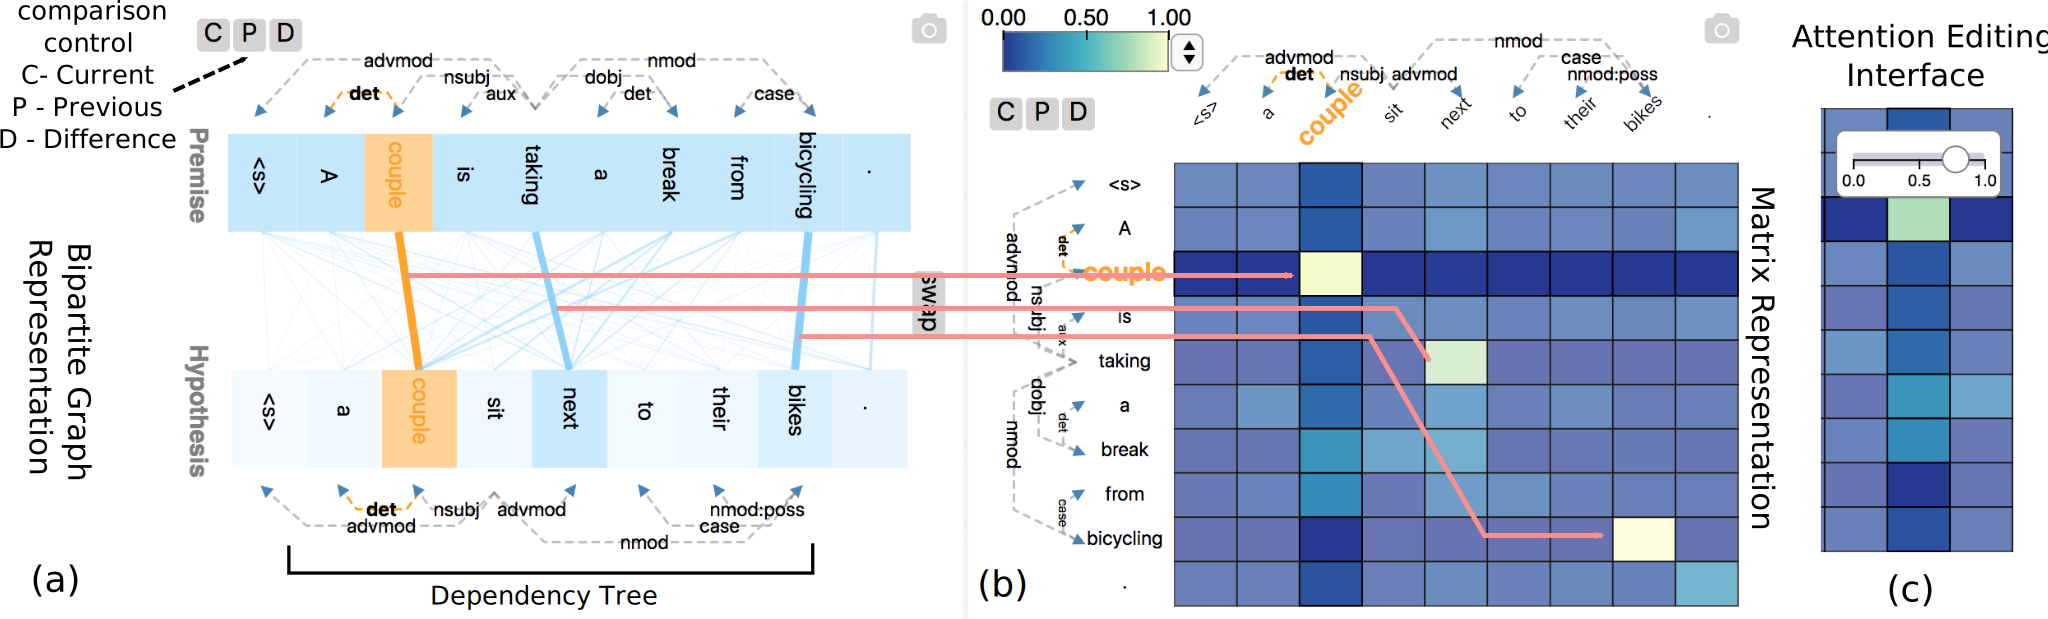
\includegraphics[width=1.0\linewidth]{attentionView}
\vspace{-6mm}
\caption{
Attention visualization. In the graph attention view (a), a bipartite graph encoding is adopted, in which the edge thickness corresponds to the attention value. In the matrix attention view (b), the entries of $i^{th}$ row represent the probabilities of words in hypotheses align to the $i^{th}$ word in the premise.
The user can alter the attention values via the pop-up interface illustrated in (c).
We overlay the dependency tree ($a_1$) grammar structure to highlight important words and simplify complex sentence to reduce clutter (d-e).
In (f), we show the difference between two attention matrix (the comparison feature is controlled by the buttons in the top left of all attention plots ($a_2$) ).
}
\label{fig:attentionVis}
\end{figure*}

\subsection{Attention View}
\label{sec:attention}
As discussed in Section~\ref{sec:attention}, the attention is the only intermediate layer in the network that provides interpretable information for domain experts to infer the inner mechanisms of the model.
%
Intuitively, the attention captures the alignment of words between input sentences. For the NLI model examined in this work, the attention is represented as a matrix, in which the entries in the $i^{th}$ row corresponds to the probabilities of words in the hypotheses align to the $i^{th}$ word in the premise.

As illustrated in Fig.~\ref{fig:attentionVis}, we employ two visual encodings for visualizing attention. In the graph attention view (Fig.~\ref{fig:attentionVis}(a)), a bipartite graph encoding is adopted, in which the edge thickness corresponds to the attention value. The color of rectangle text block encodes the sum of all edge values connect to it (darker shade of blues correspond to higher values).
%
The graph view is good for highlighting the most dominate alignments. However, if many attention values are high, the edges may become cluttered lead to less effective visualization. Also, if the sentence structures between premise and hypothesis are drastically different, we are likely to see the prominent edges cross each other, which can also lead to confusing and misleading visual patterns.

The matrix attention view (Fig.~\ref{fig:attentionVis}(b)), despite being more verbose and less efficient in highlighting the dominant alignment, do not have similar shortcomings. Together, they complement each other and provide the same information from different perspectives. As illustrated by the pink arrow line, we can see how the same attention value is visualization in both the graph and the matrix view.
To help the user recognize the correspondence during the exploration, we enable the linkage between highlight actions in both views.

To support the ability to perturb the attention values (\textbf{T2}), we include the attention editing functionality. The attention matrix view is the most suitable place to conduct the edit operation since it provides a direct mapping of attention value.
As we can see in Fig.~\ref{fig:attentionVis}(c), when a user clicks the cell of the matrix, a sider will pop up for customizing the attention value (as the user edit the value, each row is automatically normalized).
%
As illustrated in Fig.~\ref{fig:attentionVis}($a_{2}$)(f), we allow the user to compare currently and previously displayed attentions by computing and visualizing their difference.


Even though the attention does not explicitly encode any grammar, they often highlight essential words in the sentence structure.
%
To help the researcher better understand the relationship between attention and sentence structure, as illustrated in Fig.~\ref{fig:attentionVis}($a_{1}$), we overlay the grammar dependency tree~\cite{Nivre2005} structure next to the sentence.
%
Since the dependency tree encodes the word importance information in a hierarchical matter, it is very suitable for sentence simplification task.
Therefore, we utilize the grammar dependency tree to simplify the attention representations to combat the visual clutter when examining long sentences (see Fig.~\ref{fig:attentionVis}(d)).
A simplfication example is show in  Fig.~\ref{fig:attentionVis}(d)(e)(f).


%\subsubsection{Attention visualization challenges}
% \begin{itemize}
% 	\item Why we need two different visual encoding to visualize attention? bipartite visualization more easier to highlight the
% 	\item long sentence, collapse
% 	\item quickly compare the alignment information with the sentence's linguistic structure.
% \end{itemize}


% \subsection{Interpret Attention Via Model Perturbation}
